\subsection{Simulatie}
\begin{figure}[h!]
    \centering
    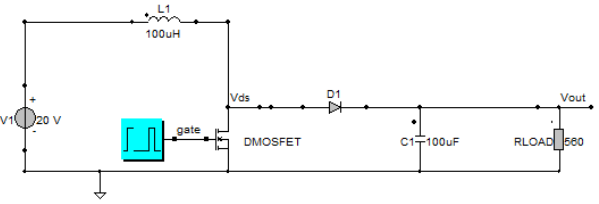
\includegraphics[width=1\linewidth]{img/hfd1/Schema voor de simulatie van een boostconverter.png}
    \caption{Schema voor de simulatie van een boostconverter}
    \label{fig:Schema voor de simulatie van een boostconverter}
\end{figure}
\begin{table}[h!]
\centering
\begin{tabular}{|l|c|c|c|}
\hline
\textbf{Duty Cycle (\%)} & \textbf{Vuit (V) Rl=1MEG (onbelast)} & \textbf{Vuit (V) Rl=560 Ohm} & \textbf{Vuit (V) Rl=56 Ohm} \\ \hline
10 & 42.77 & 42.57 & 41.98 \\ \hline
20 & 48.41 & 48.01 & 47.26 \\ \hline
40 & 65.02 & 64.34 & 62.91 \\ \hline
50 & 77.95 & 77.23 & 75.25 \\ \hline
75 & 139.54 & 138.83 & 132.72 \\ \hline
\end{tabular}
\caption{Uitgangsspanningen Vuit bij verschillende belasting en duty cycles}
\end{table}
Uit de simulaties blijkt dat de uitgangsspanning toeneemt met een hogere duty cycle, zoals verwacht bij een boostconverter. De belasting beïnvloedt de spanning: bij zwaardere belasting daalt de uitgangsspanning licht. De resultaten komen goed overeen met de theorie en tonen de correcte werking van de schakeling. De wet van Kirchhoff en \(UL = L \cdot \frac{dI}{dt}\) zijn duidelijk waarneembaar in de stroom- en spanningsgolfvormen.

\subsubsection{10\% dutycycle, 1 MEG ohm load}
\begin{figure}[h!]
    \centering
    \begin{subfigure}[b]{0.3\linewidth}
        \centering
        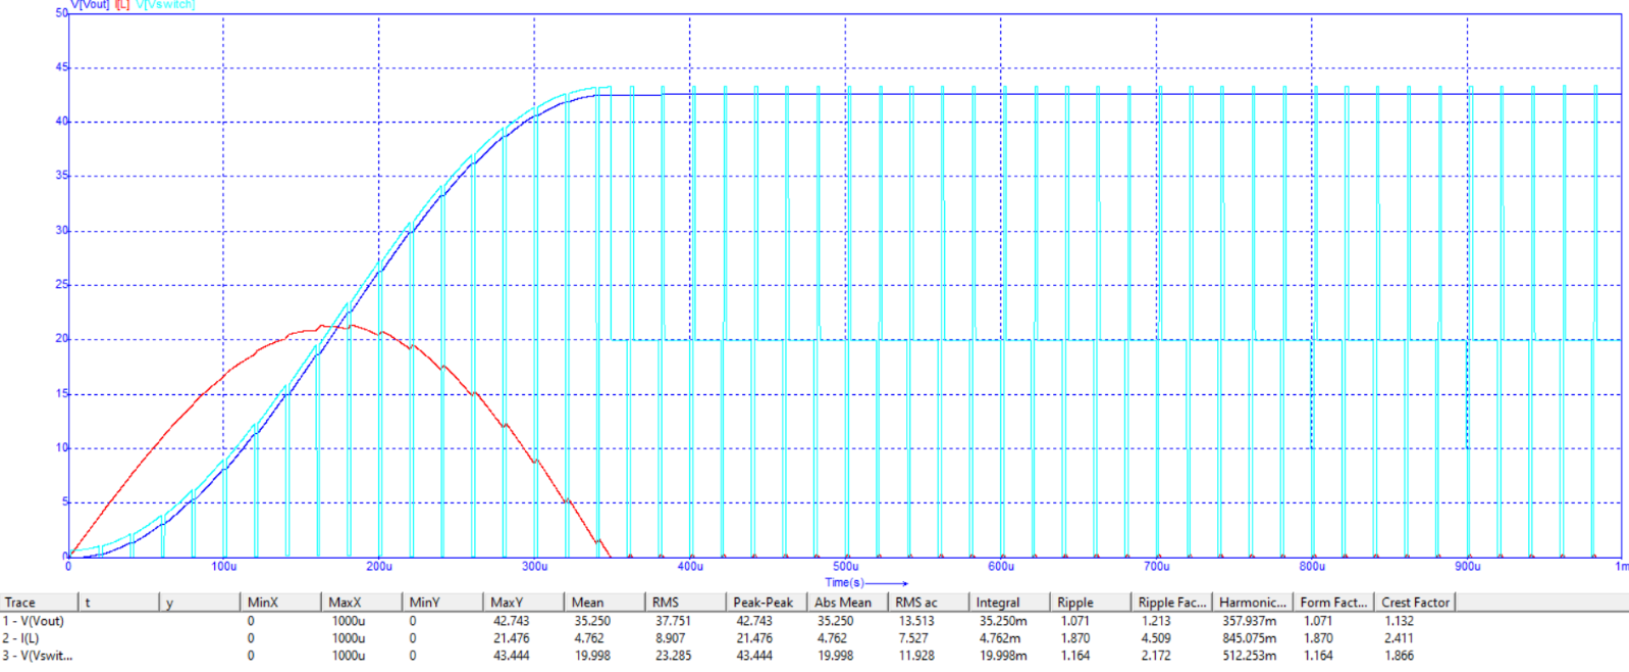
\includegraphics[width=\linewidth]{img/hfd1/hfd1-10pduty-1MEG-INDUCTOR.png}
        \caption{Spoelstroom}
        \label{fig:inductor}
    \end{subfigure}
    \hfill
    \begin{subfigure}[b]{0.3\linewidth}
        \centering
        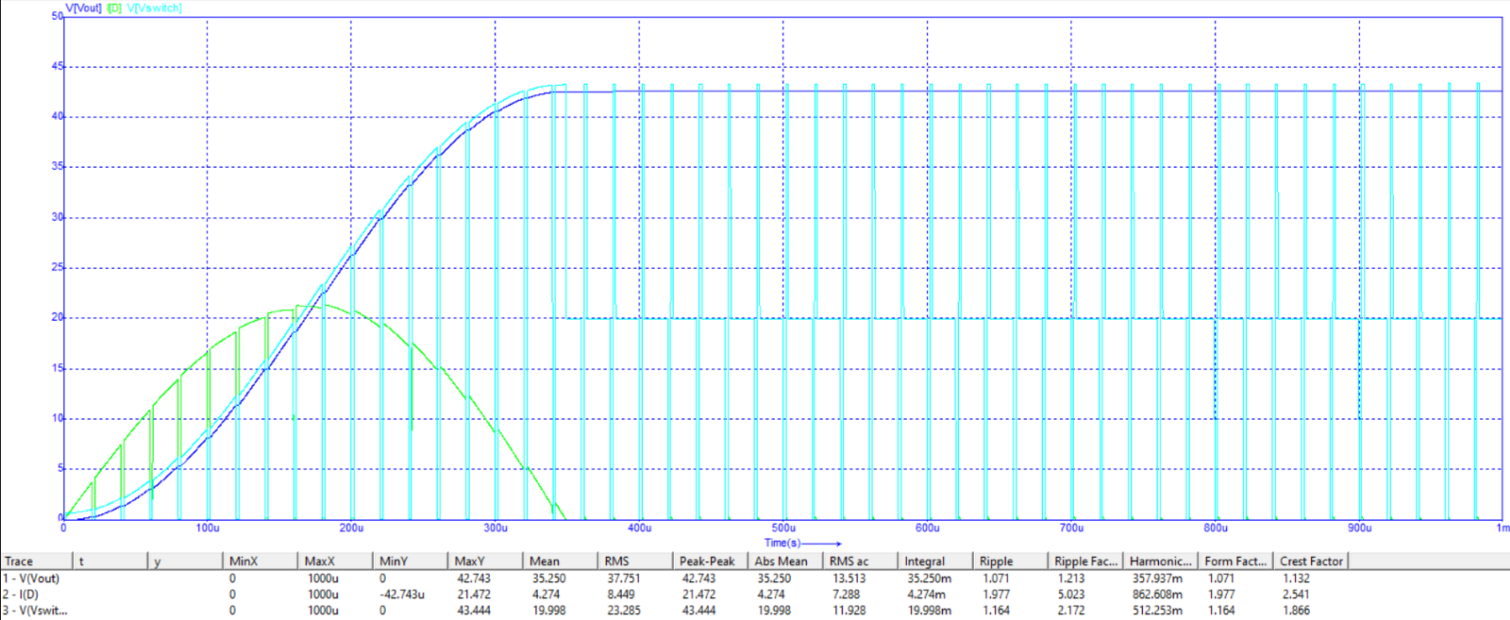
\includegraphics[width=\linewidth]{img/hfd1/hfd1-10pduty-1MEG-DIODE.png}
        \caption{Diodestroom}
        \label{fig:diode}
    \end{subfigure}
    \hfill
    \begin{subfigure}[b]{0.3\linewidth}
        \centering
        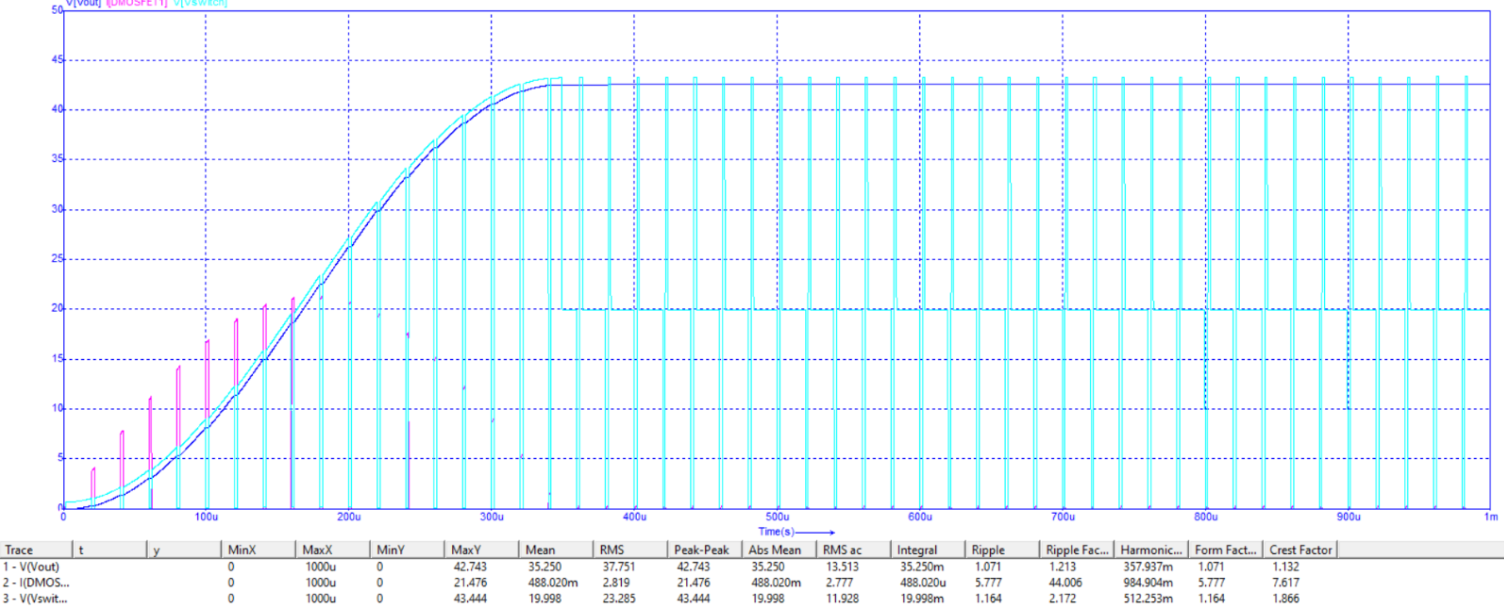
\includegraphics[width=\linewidth]{img/hfd1/hfd1-10pduty-1MEG-DMOSFET.png}
        \caption{Mosfetstroom}
        \label{fig:mosfet}
    \end{subfigure}
    
    \caption{Vergelijking van stroom en spanning bij verschillende componenten met een weerstand van 1M\(\Omega\) en duty cycle van 10\%.}
    \label{fig:componenten}
\end{figure}




\subsubsection{40\% duty cycle, 560 ohm load}
\begin{figure}[h!]
    \centering
    \begin{subfigure}[b]{0.3\linewidth}
        \centering
        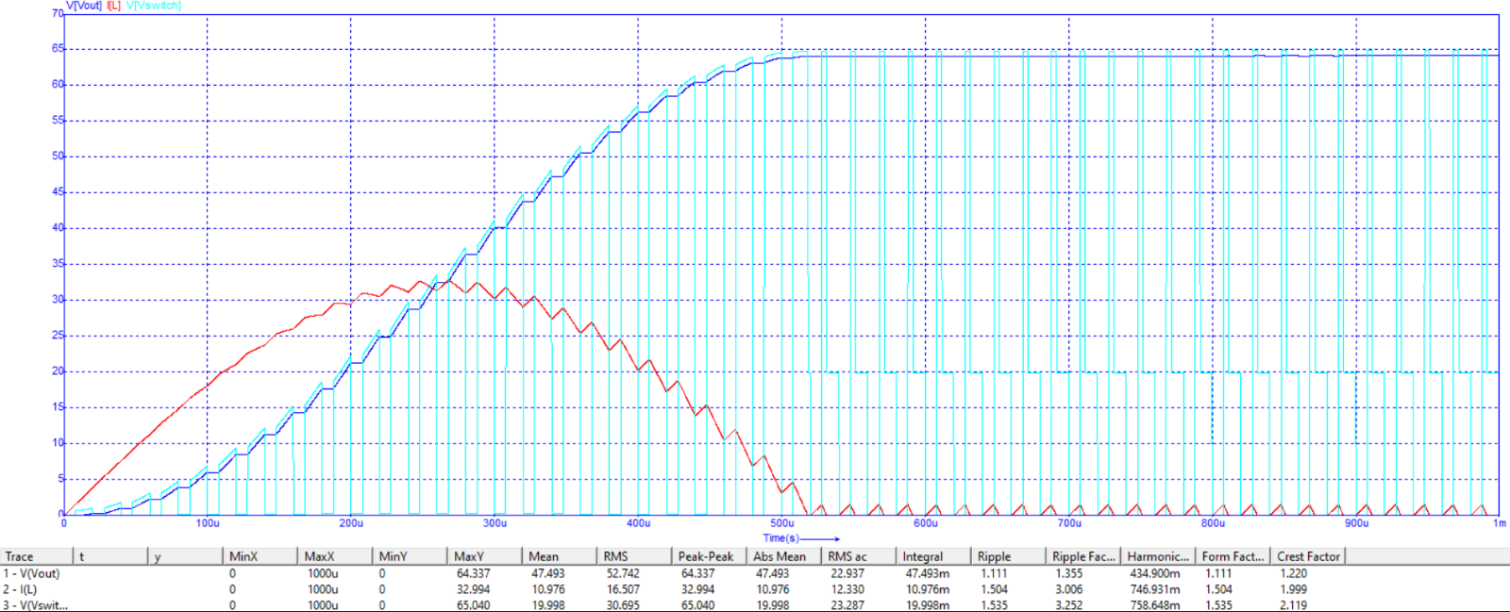
\includegraphics[width=\linewidth]{img/hfd1/hfd1-40pduty-560-INDUCTOR.png}
        \caption{Spoelstroom}
        \label{fig:inductor40}
    \end{subfigure}
    \hfill
    \begin{subfigure}[b]{0.3\linewidth}
        \centering
        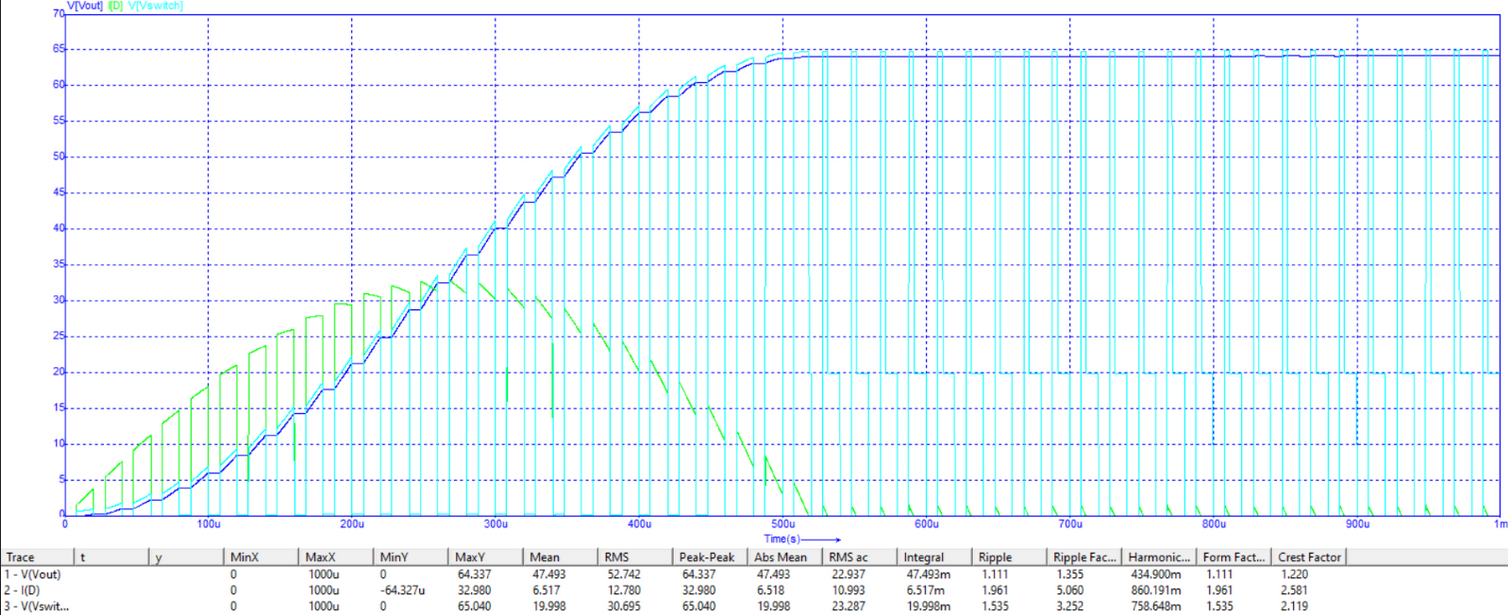
\includegraphics[width=\linewidth]{img/hfd1/hfd1-40pduty-560-DIODE.png}
        \caption{Diodestroom}
        \label{fig:diode40}
    \end{subfigure}
    \hfill
    \begin{subfigure}[b]{0.3\linewidth}
        \centering
        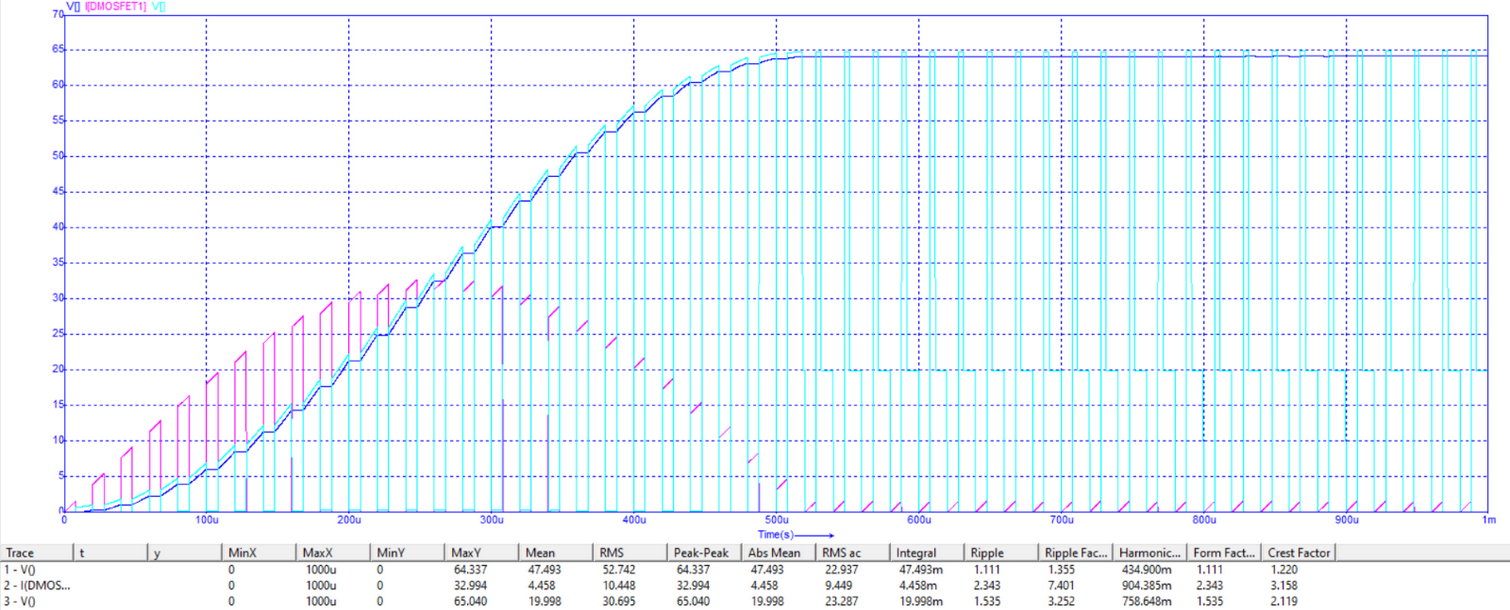
\includegraphics[width=\linewidth]{img/hfd1/hfd1-40pduty-560-MOSFET.png}
        \caption{Mosfetstroom}
        \label{fig:mosfet40}
    \end{subfigure}
    
    \caption{Vergelijking van stroom en spanning bij verschillende componenten met een weerstand van 560\(\Omega\) en duty cycle van 40\%.}
    \label{fig:componenten40}
\end{figure}




\subsubsection{75\% duty cycle, 56 ohm load}

\begin{figure}[h!]
    \centering
    \begin{subfigure}[b]{0.3\linewidth}
        \centering
        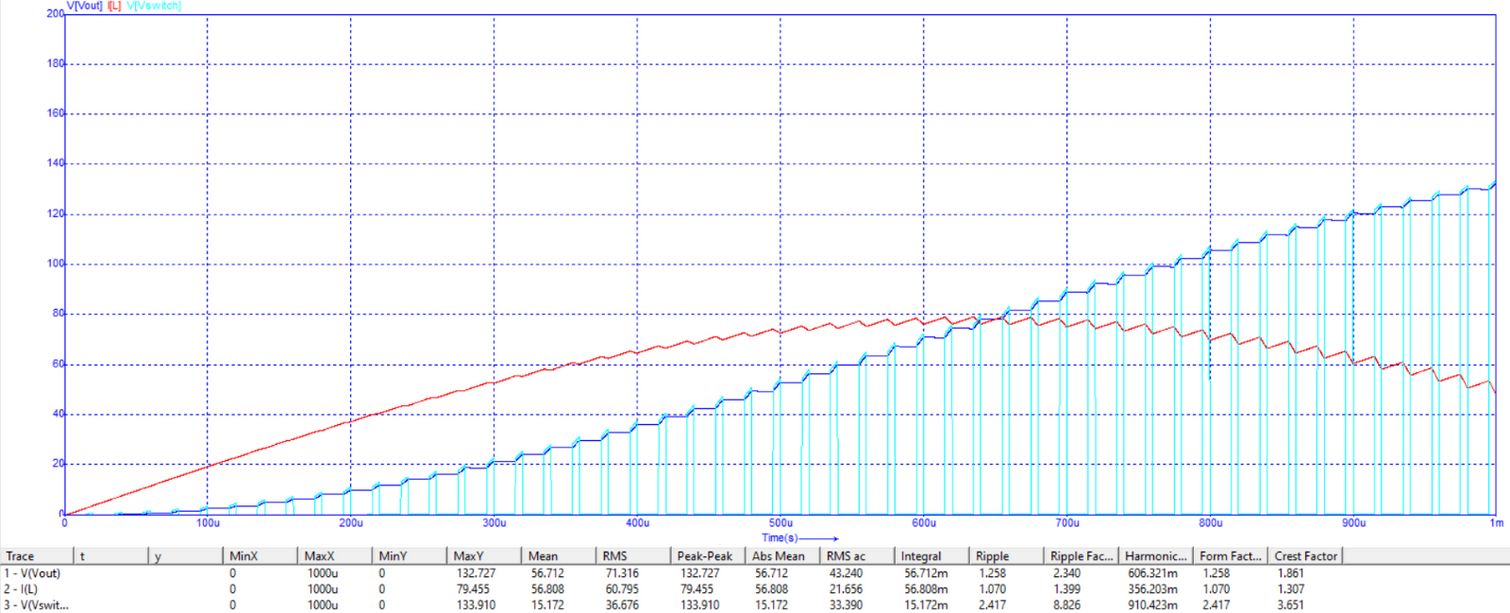
\includegraphics[width=\linewidth]{img/hfd1/hfd1-75pduty-56-INDUCTOR.png}
        \caption{Spoelstroom}
        \label{fig:inductor75}
    \end{subfigure}
    \hfill
    \begin{subfigure}[b]{0.3\linewidth}
        \centering
        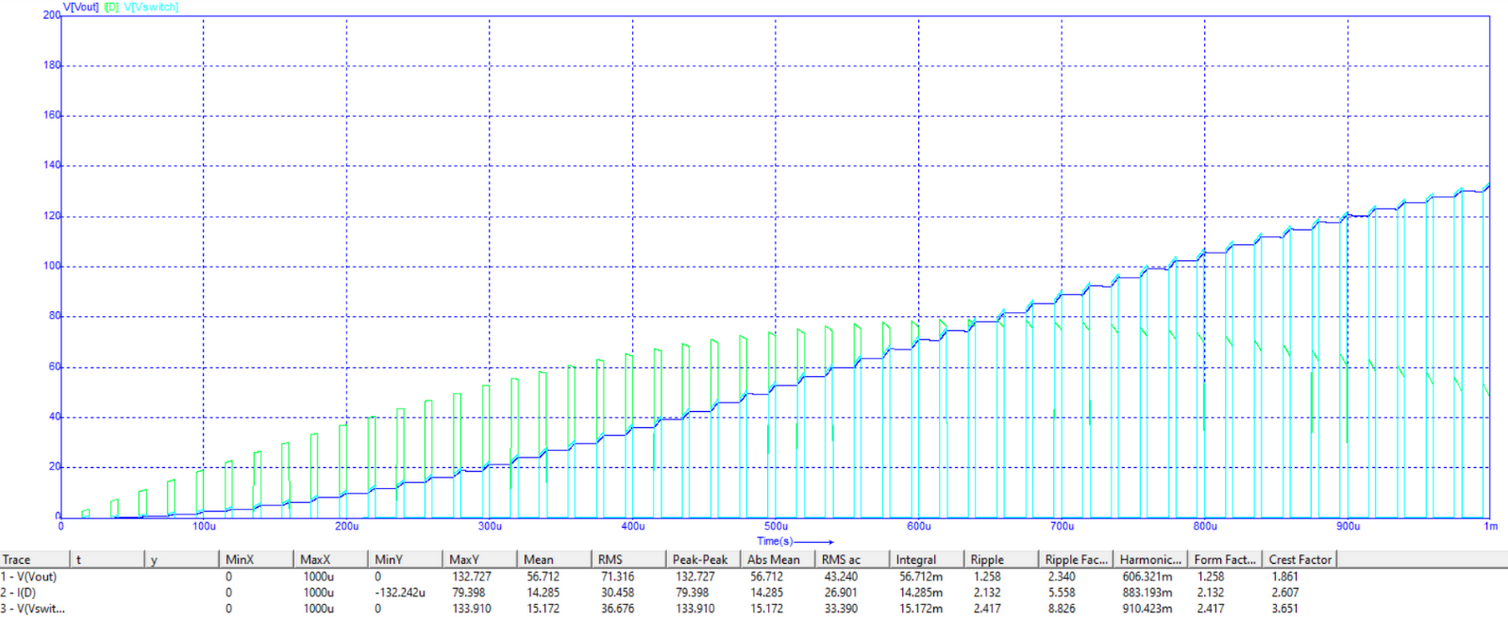
\includegraphics[width=\linewidth]{img/hfd1/hfd1-75pduty-56-DIODE.png}
        \caption{Diodestroom}
        \label{fig:diode75}
    \end{subfigure}
    \hfill
    \begin{subfigure}[b]{0.3\linewidth}
        \centering
        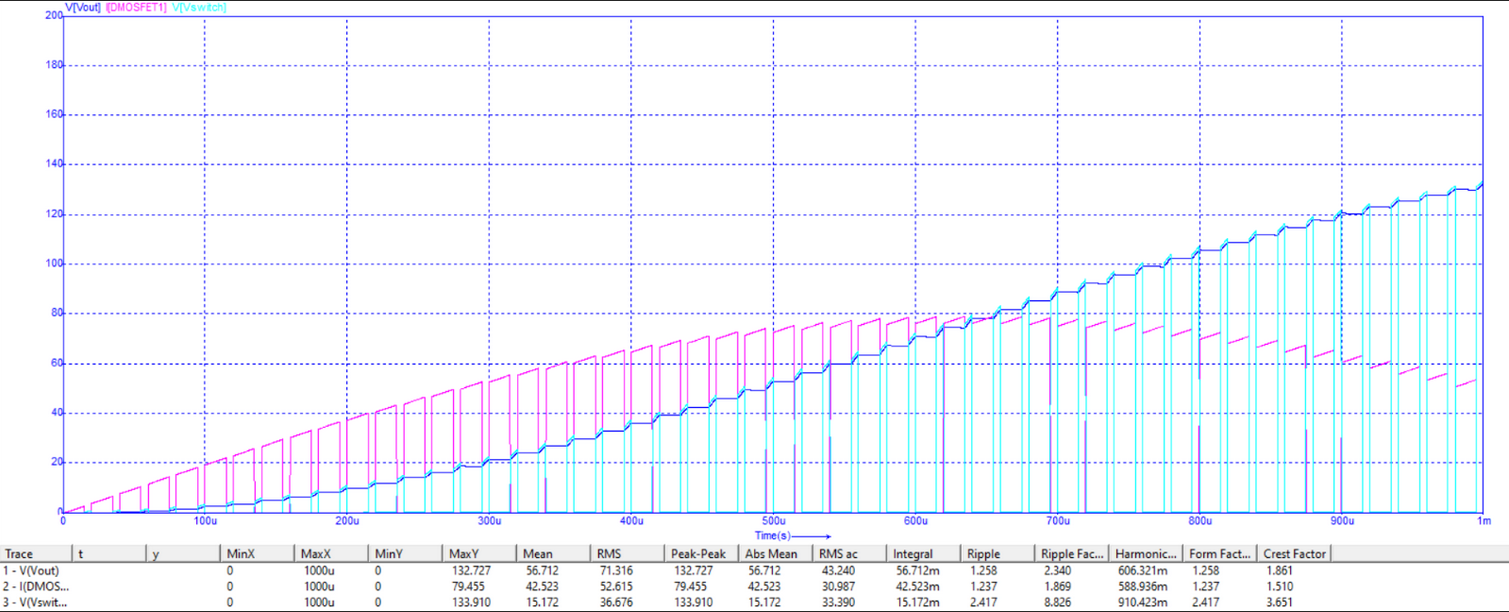
\includegraphics[width=\linewidth]{img/hfd1/hfd1-75pduty-56-DMOSFET.png}
        \caption{Mosfetstroom}
        \label{fig:mosfet75}
    \end{subfigure}
    
    \caption{Vergelijking van stroom en spanning bij verschillende componenten met een weerstand van 56\(\Omega\) en duty cycle van 75\%.}
    \label{fig:componenten75}
\end{figure}

[HIER MOET NOG UITLEG KOMEN]